\documentclass[12pt]{beamer}
\newenvironment{ConCodigo}[1]
  {\begin{frame}[fragile,environment=ConCodigo]{#1}}
  {\end{frame}}
\graphicspath{{Imagenes/}{../Imagenes/}}
\usepackage[utf8]{inputenc}
\usepackage[spanish]{babel}
\usepackage{hyperref}
\usepackage{etex}
%\reserveinserts{28}
\usepackage{amsmath}
\usepackage{amsthm}
\usepackage{mathtools}
\usepackage{multicol}
\usepackage{multirow}
\usepackage{tabulary}
\usepackage{booktabs}
\usepackage{nccmath}
\usepackage{physics}
\usepackage{biblatex}
\usepackage[outdir=./]{epstopdf}
%\epstopdfsetup{outdir=./}
\usepackage{graphicx}
%\usepackage{enumitem,xcolor}
\usepackage{siunitx}
%\sisetup{scientific-notation=true}
%\usepackage{fontspec}
\usepackage{lmodern}
\usepackage{float}
\usepackage[format=hang, font=footnotesize, labelformat=parens]{caption}
\usepackage[autostyle,spanish=mexican]{csquotes}
\usepackage{standalone}
\usepackage{blkarray}
\usepackage{algorithm}
\usepackage{algorithmic}
\usepackage{tikz}
\usepackage[siunitx, RPvoltages]{circuitikz}
\usetikzlibrary{arrows,patterns,shapes}
\usetikzlibrary{decorations.markings}
\usetikzlibrary{arrows}
\usepackage{color}
\usepackage{xcolor}
%\usepackage{beton}
%\usepackage{euler}
%\usepackage[T1]{fontenc}
\usepackage[sfdefault]{roboto}  %% Option 'sfdefault' only if the base font of the document is to be sans serif
\usepackage[T1]{fontenc}
\renewcommand*\familydefault{\sfdefault}
\DeclareGraphicsExtensions{.pdf,.png,.jpg}
\usepackage{hyperref}
\renewcommand {\arraystretch}{1.5}
\newcommand{\python}{\texttt{python}}
\usefonttheme[onlymath]{serif}
\setbeamertemplate{navigation symbols}{}
\usetikzlibrary{patterns}
\usetikzlibrary{decorations.markings}
\tikzstyle{every picture}+=[remember picture,baseline]
%\tikzstyle{every node}+=[inner sep=0pt,anchor=base,
%minimum width=2.2cm,align=center,text depth=.15ex,outer sep=1.5pt]
%\tikzstyle{every path}+=[thick, rounded corners]
\setbeamertemplate{caption}[numbered]
\newcommand{\ptm}{\fontfamily{ptm}\selectfont}
%Se usa la plantilla Warsaw modificada con spruce
\mode<presentation>
{
  \usetheme{Warsaw}
  \setbeamertemplate{headline}{}
  \useoutertheme{default}
  \usecolortheme{albatross}
  \setbeamercovered{invisible}
}
% \AtBeginSection[]
% {
% \begin{frame}<beamer>{Contenido}
% \normalfont\mdseries
% \tableofcontents[currentsection]
% \end{frame}
% }

\include{pre_codigo}
\title{Ecuaciones diferenciales parciales}
\subtitle{Curso de Física Computacional}
\author{M. en C. Gustavo Contreras Mayén}
\begin{document}
\maketitle
\fontsize{14}{14}\selectfont
\spanishdecimal{.}
\begin{frame}{Contenido}
\tableofcontents[pausesections]
\end{frame}
\section{Introducción}
\begin{frame}
Muchos fenómenos físicos se pueden modelar matemáticamente con ecuaciones diferenciales.
\\
\medskip
Cuando la función que se está estudiando implica dos o más variables independientes, la ecuación diferencial es generalmente una ecuación diferencial parcial (EDP).
\\
\medskip
Dado que las funciones de varias variables son intrínsicamente más complicadas que las de una variable, las EDP puede dar lugar  a algunos de los más difíciles problemas numéricos.
\end{frame}
\begin{frame}
Las cantidades físicas como la temperatura y la presión varían continuamente tanto en tiempo y espacio.
\\
\medskip
Como hemos aprendido en la carrera, usamos una función o campo  $U(x, y, z, t)$ para describir esas cantidades y deben de considerarse variaciones independientes de tiempo y espacio.
\end{frame}
\begin{frame}
El cambio en la variable tiempo genera cambios en  $U (x, y, z, t)$ en cualquier posición y ésta a su vez afecta a los puntos vecinos.
\\
\medskip
Esto significa que las ecuaciones son dinámicas y describen la dependencia de $U$ en las cuatro variables independientes, por lo que debería de escribirse en términos de derivadas parciales; tenemos una ecuación diferencial parcial (\textit{EDP})
\end{frame}
\section{Forma General de una EDP}
\begin{frame}
La forma más general de una Ecuación Diferencial Parcial (EDP) de segundo orden
\[ A \dfrac{\partial^{2} U}{\partial x^{2}} + 2B \dfrac{\partial^{2} U}{\partial x \partial y} + C \dfrac{\partial^{2} U}{\partial y^{2}} + D \dfrac{\partial U}{\partial x} + E \dfrac{\partial U}{\partial y} = F \]
Donde A, B, C y F son funciones arbitrarias
de x e y
\end{frame}
\section{Tipos de EDP}
\begin{frame}
\[ A \dfrac{\partial^{2} U}{\partial x^{2}} + 2B \dfrac{\partial^{2} U}{\partial x \partial y} + C \dfrac{\partial^{2} U}{\partial y^{2}} + D \dfrac{\partial U}{\partial x} + E \dfrac{\partial U}{\partial y} = F \]
\\
\medskip
Se pueden clasificar las EDP en tres categorías, si sucede que:
\begin{enumerate}
\item Elíptica si: $d = AC - B^{2} > 0$
\item Parabólica si: $d = AC - B^{2} = 0$
\item Hiperbólica si: $d = AC – B^{2}  < 0$  
\end{enumerate}
\end{frame}
\begin{frame}
\frametitle{EDP tipo Elíptico $d = AC - B^{2} > 0$}
La ecuación en de Poisson en 2D, donde $u$ representa una función de potencial eléctrico, y $\rho$ representa un término fuente.
\[ \dfrac{\partial^{2} u}{\partial x^{2}} + \dfrac{\partial^{2} u}{\partial y^{2}} = - \dfrac{\rho(x,y)}{\epsilon_{0}} \]
\end{frame}
\begin{frame}
\frametitle{EDP Tipo Parabólico $AC-B^{2}=0$}
La ecuación de difusión, donde $D$ representa el coeficiente de difusión,  $u$ puede representar cualquier cantidad con propiedades difusivas, como la temperatura.
\[ D \dfrac{\partial^{2} u}{\partial x^{2}} = \dfrac{\partial u}{\partial x} \]
\end{frame}
\begin{frame}
\frametitle{EDP Tipo Hiperbólico $AC-B^{2}<0$}
La ecuación de onda unidimensional
\[ \dfrac{\partial^{2} u}{\partial x^{2}} = \dfrac{1}{v^{2}} \dfrac{\partial^{2} u}{\partial t^{2}} \]
\\
\medskip
donde $u$ es la amplitud de onda y $v$ su velocidad de propagación.
\end{frame}
\section{Problemas de valores iniciales}
\begin{frame}
\frametitle{Problema de valores iniciales}
Este tipo de problemas es en general un problema de evolución en el tiempo, en el que las condiciones iniciales se refieren al estado del sistema en el tiempo $t=0$
\end{frame}
\section{Problema de condiciones de frontera}
\begin{frame}
\frametitle{Problema de condiciones de frontera}
Este tipo de problemas considera una solución estática, es decir, en muchos de los casos, nuestro sistema evolucionó en el tiempo hasta llegar a un estado estable, en estas condiciones lo que nos interesa es el valor de nuestra solución en las fronteras de la región de interés.
\end{frame}
\section{Tipos de condiciones}
\begin{frame}
\frametitle{Tipos de condiciones}
\begin{itemize}
\item \textbf{Dirichlet}: El valor de la función está especificado en la frontera.
\item \textbf{Neumann}: El valor de la derivada normal (gradiente) de la función está especificado en la frontera.
\item \textbf{Cauchy}: El valor de la función y de la derivada normal están especificados en la frontera.
\end{itemize}
\end{frame}
\begin{frame}
\frametitle{Relación entre condiciones de frontera y solución de EDP}
\fontsize{8}{8}\selectfont
\begin{tabular}{p{2cm} | l l l}
	Condición                & Elíptica & Hiperbólica & Parabólica \\ \hline
	Dirichlet superficie abierta &              &                 & Unica y estable 1D \\ \hline
	Dirichlet superficie cerrada & Unica y estable &                 &  \\ \hline
	Neumann superficie abierta &              &                 & Unica y estable 1D \\ \hline
	Neumann superficie cerrada & Unica y estable &                 & \\ \hline
	Cauchy superficie abierta &  Sin sentido físico            & Unica y estable &  \\ \hline
	Cauchy superficie cerrada &              &                 &  \\ \hline
\end{tabular}
\end{frame}
\begin{frame}
\frametitle{Problema de condición inicial}
\begin{center}
\begin{tikzpicture}[scale=0.9]
\draw [fill=gray!50, thin] (0,0) rectangle (6,4);
\draw [gray](0,4) -- (6,4);
\draw [font=\normalsize](3,2) node {La solución se determina aquí };
\draw (0,-0.5) [font=\tiny] node {$x=-\dfrac{L}{2}$};
\draw (6,-0.5) [font=\tiny] node {$x= \dfrac{L}{2}$};
\draw [arrows=->] (3,-1) -- (3,0);
\draw [font=\tiny](3,-1.2) node {Condiciones iniciales $f(x,t=0) = F(x)$ };
\draw [arrows=->] (-1,1) -- (0,2.5);
\draw [font=\tiny](-1.3,0.8) node {Condiciones de frontera};
\draw [font=\tiny](-1.3,0.5) node {$f(x=-L/2,t)=f_{1}$};
\draw [arrows=->] (7,1) -- (6,2.5);
\draw [font=\tiny](7.3,0.8) node {Condiciones de frontera};
\draw [font=\tiny](7.3,0.5) node {$f(x=-L/2,t)=f_{2}$};
\draw [font=\tiny](-0.4,0) node {$t=0$};
\draw [arrows=->] (7.5,4) -- (7.5,5);
\draw [arrows=->] (7.5,4) -- (8.5,4);
\draw [font=\tiny](7.35,5) node {t};
\draw [font=\tiny](8.6,4) node {x};
\end{tikzpicture}
\end{center}
\end{frame}
\begin{frame}
\frametitle{Problema de condiciones de frontera}
\begin{center}
\begin{tikzpicture}[scale=0.9]
\draw [fill=gray!50, thin] (0,0) rectangle (6,4);
\draw [font=\normalsize](3,2) node {La solución se determina aquí };
\draw (0,-0.5) [font=\tiny] node {$x=0$};
\draw (6,-0.5) [font=\tiny] node {$x= L_{x}$};
\draw [arrows=->] (3,-1) -- (3,0);
\draw [font=\tiny](3,-1.2) node {Condiciones de frontera};
\draw [arrows=->] (3,5) -- (3,4);
\draw [font=\tiny](3,5.2) node {Condiciones de frontera};
\draw [arrows=->] (-1,1) -- (0,2.5);
\draw [font=\tiny](-1.3,0.8) node {Condiciones de frontera};
\draw [arrows=->] (7,1) -- (6,2.5);
\draw [font=\tiny](7.3,0.8) node {Condiciones de frontera};
\draw [font=\tiny](-0.5,0.1) node {$y=0$};
\draw [font=\tiny](-0.5,4) node {$y=L_{y}$};
\draw [arrows=->] (7.5,4) -- (7.5,5);
\draw [arrows=->] (7.5,4) -- (8.5,4);
\draw [font=\tiny](7.35,5) node {y};
\draw [font=\tiny](8.6,4) node {x};
\end{tikzpicture}
\end{center}
\end{frame}
\section{Problema de potencial eléctrico}
\begin{frame}
\fontsize{14}{14}\selectfont
\frametitle{Problema de potencial eléctrico}
Nuestro problema es calcular el potencial eléctrico para todos los puntos que están dentro del cuadro.
\\
\medskip
La parte inferior y las orillas de la región están unidos y conectados a "tierra", mientras que en la parte superior tenemos un cable conectado a una fuente de voltaje de 100 Volts.
\begin{center}
\begin{tikzpicture}[scale=0.6]
\draw [line width=3pt] (0,3) -- (4,3);
\draw [font=\tiny](2,3.5) node {100 V};
\draw [font=\tiny](2,-0.3) node {0 V};
\draw [dashed](0,2.8) -- (0,0);
\draw [dashed](0,0) -- (4,0);
\draw [dashed](4,0) -- (4,2.8);
\draw (0.5,0) -- (0.5,-0.3);
\draw (0.2,-0.3) -- (0.8,-0.3);
\draw (0.3,-0.4) -- (0.7,-0.4);
\draw (0.4,-0.5) -- (0.6,-0.5);
\end{tikzpicture}
\end{center}
\end{frame}
\begin{frame}
\frametitle{EDP Elíptica, la ecuación de Laplace}
Consideremos que tenemos un cuadrado completo para nuestro problema, de tal forma que tenemos unos aislantes que cierran la forma.
\\
\medskip
Dado que conocemos los valores de potencial, tenemos un problema con condiciones de Neumann en la frontera, por lo que la solución es única y estable.
\end{frame}
\begin{frame}
Sabemos de la teoría electrodinámica que el potencial eléctrico $U(x)$ alrededor de una carga estática, satisface la ecuación de Poisson:
\[ \nabla^{2} U(x) = - 4 \pi \rho(x) \]
donde $\rho(x)$ es la densidad de carga.
\end{frame}
\begin{frame}
En las regiones espaciales sin carga, es decir $\rho(x)=0$, el potencial satisface la ecuación de Laplace:
\[ \nabla^{2} U(x) = 0\]
\end{frame}
\begin{frame}
Resolviendo las ecuaciones en 2-D en coordenadas rectangulares:
\[ \dfrac{\partial^{2} U(x,y)}{\partial x^{2}} + \dfrac{\partial^{2} U(x,y)}{\partial y^{2}}  = \left\lbrace \begin{array}{l}
0 \\
- 4\pi \rho(x)
\end{array} \right. \]
\end{frame}
\begin{frame}
\fontsize{14}{14}\selectfont
\frametitle{Solución: Método de diferencias finitas}
Para resolver nuestra ecuación 2-D numéricamente, dividimos el espacio en una malla y buscamos la solución para $U$ en cada una de ellas.
\\
\medskip
Como expresaremos derivadas en términos de diferencias finitas de los valores de $U$ para cada elemento de la malla, este método se llama precisamente de diferencias finitas. Un método más eficiente pero a la vez más complicado es la técnica del elemento finito que resuelve la EDP para pequeños elementos geométricos.
\end{frame}
\begin{frame}
\frametitle{División de la región de trabajo}
El algoritmo para la ecuación de Laplace: el potencial en un punto $(x,y) = (i,j)$ $\Delta$ es igual al promedio de los valores de potencial de los cuatro puntos vecinos, los nodos con los centros en blanco, corresponden a los valores de potencial constante sobre la frontera.
\end{frame}
\begin{frame}
\begin{center}
\begin{tikzpicture}[scale=0.9]
\draw [arrows=->] (0,8) -- (8.4,8) ;
\draw [arrows=->] (0,8) -- (0,0.7);
\draw [font=\tiny] (8.2,8.2) node {x};
\draw [font=\tiny] (-0.3,1) node {y};
\foreach \x in {0,1,2,3,4,5,6,7,8} \draw [fill](\x,8) circle (0.08);
\foreach \x in {0,1,2,3,4,5,6,7,8} \draw [fill=white](\x,8) circle (0.03);
\foreach \x in {0,1,2,3,4,5,6,7,8} \draw [fill](\x,1) circle (0.08);
\foreach \x in {0,1,2,3,4,5,6,7,8} \draw [fill=white](\x,1) circle (0.03);
\foreach \x in {0,1,2,3,4,5,6,7} \draw [fill](0, \x) circle (0.08);
\foreach \x in {0,1,2,3,4,5,6,7} \draw [fill=white](0, \x) circle (0.03);
\foreach \x in {0,1,2,3,4,5,6,7} \draw [fill](8, \x) circle (0.08);
\foreach \x in {0,1,2,3,4,5,6,7} \draw [fill=white](8, \x) circle (0.03);
\foreach \x in {1,2,3,4,5,6,7} \draw [fill](\x, 2) circle (0.04);
\foreach \x in {1,2,3,4,5,6,7} \draw [fill](\x,3) circle (0.04);
\foreach \x in {1,2,3,4,5,6,7} \draw [fill](\x,4) circle (0.04);
\foreach \x in {1,2,3,4,5,6,7} \draw [fill](\x,5) circle (0.04);
\foreach \x in {1,2,3,4,5,6,7} \draw [fill](\x,6) circle (0.04);
\foreach \x in {1,2,3,4,5,6,7} \draw [fill](\x,7) circle (0.04);
\draw [fill=white](4,4) circle(0.3);
\draw [fill=white](3,4) circle(0.3);
\draw [fill=white](5,4) circle(0.3);
\draw [fill=white](4,3) circle(0.3);
\draw [fill=white](4,5) circle(0.3);
\draw [font=\tiny] (4,4) node {i,j};
\draw [font=\tiny] (3,4) node {i-1,j};
\draw [font=\tiny] (5,4) node {i+1,j};
\draw [font=\tiny] (4,3) node {i,j-1};
\draw [font=\tiny] (4,5) node {i,j+1};
\draw [arrows=->] (3.3,4) -- (3.7,4);
\draw [arrows=->] (4.7,4) -- (4.3,4);
\draw [arrows=->] (4,3.3) -- (4,3.7);
\draw [arrows=->] (4,4.7) -- (4,4.3);
\end{tikzpicture}
\end{center}
\end{frame}
\begin{frame}
\fontsize{14}{14}\selectfont
Usaremos el algoritmo de diferenciación hacia adelante. Sumamos las dos series de Taylor para el potencial: a la derecha e izquierda de $(x,y)$ así como para arriba y abajo de $(x,y)$:
\begin{eqnarray*}
U(x+\Delta x,y) = U(x,y) + \dfrac{\partial U}{\partial x} \Delta x + \dfrac{1}{2} \dfrac{\partial^{2} U}{\partial x^{2}} (\Delta x)^{2} + \ldots \\
U(x -\Delta x,y) = U(x,y) - \dfrac{\partial U}{\partial x} \Delta x + \dfrac{1}{2} \dfrac{\partial^{2} U}{\partial x^{2}} (\Delta x)^{2} - \ldots \\
\end{eqnarray*}
\end{frame}
\begin{frame}
\fontsize{14}{14}\selectfont
Todos los términos impares se cancelan, al sumar las ecuaciones obtendremos una aproximación por diferencias centrales para las segunda derivada parcial:
\begin{eqnarray*}
\dfrac{\partial^{2} U(x,y)}{\partial x^{2}} \simeq \dfrac{U(x+\Delta x, y) + U(x-\Delta x,y)-2U(x,y)}{(\Delta x)^{2}} \\
\dfrac{\partial^{2} U(x,y)}{\partial y^{2}} \simeq \dfrac{U(x, y+\Delta y) + U(x,y-\Delta y)-2U(x,y)}{(\Delta y)^{2}}
\end{eqnarray*}
\end{frame}
\begin{frame}
\fontsize{14}{14}\selectfont
Al sustituir las dos ecuaciones en la ecuación de Laplace, obtenemos una expresión en diferencias finitas para la EDP:
\begin{eqnarray*}
\dfrac{U(x+\Delta x,y) + U(x-\Delta x, y) - 2U(x,y)}{(\Delta x^{2})} + {} \\
{} + \dfrac{U(x,y+\Delta y) + U(x,y-\Delta y) - 2U(x,y)}{(\Delta y)^{2}} \simeq 0
\end{eqnarray*}
\end{frame}
\begin{frame}
\fontsize{14}{14}\selectfont
Asumimos que en la malla $(x,y$ tienen el mismo espaciamiento $\Delta x =  \Delta y = \Delta$, por el que el algoritmo toma la sencilla forma:
\begin{eqnarray*}
U(x + \Delta, y)+ U(x-\Delta, y) + {} \\
U(x,y +\Delta) + U(x,y - \Delta) - 4 U(x,y)= 0
\end{eqnarray*}
La ecuación muestra una relación entre las soluciones en los cinco puntos. Cuando $U(x,y)$ se evalúa para $N_{x}$ x valores en la malla y para $N_{y}$ y valores, obtenemos un conjunto de $N_{x} \times N_{y}$ ecuaciones algebraicas lineales.
\end{frame}
\begin{frame}
\fontsize{14}{14}\selectfont
Hacemos una aproximación para $U(x,y)$
\begin{eqnarray*}
U(x,y) \simeq	\dfrac{1}{4} \left[ U(x+\Delta ,y) + U(x-\Delta,y) + \right. \\
\left. + U(x,y+\Delta) + U(x,y-\Delta) \right]
\end{eqnarray*}
En términos de posiciones discretas de la malla, las variables $x$, $y$ son:
\[ x= x_{0} + i \Delta, \hspace{1cm} y=y_{0}+ j \Delta, \hspace{0.8cm} i,j=0,1,\ldots,N_{max-1} \]
\end{frame}
\begin{frame}
\fontsize{14}{14}\selectfont
El algoritmo de diferencias finitas resulta ser:
\[ U_{i,j} = \dfrac{1}{4} [U_{i+1,j} + U_{i-1,j} + U_{i,j+1} + U_{i,j-1}] \]
\begin{center}
\begin{tikzpicture}[scale=0.6]
\draw [line width=3pt] (0,3) -- (4,3);
\draw [font=\tiny](2,3.5) node {100 V};
\draw [font=\tiny](2,-0.3) node {0 V};
\draw [dashed](0,2.8) -- (0,0);
\draw [dashed](0,0) -- (4,0);
\draw [dashed](4,0) -- (4,2.8);
\draw (0.5,0) -- (0.5,-0.3);
\draw (0.2,-0.3) -- (0.8,-0.3);
\draw (0.3,-0.4) -- (0.7,-0.4);
\draw (0.4,-0.5) -- (0.6,-0.5);
\end{tikzpicture}
\end{center}
\end{frame}
\section{Implementando el código}
\begin{frame}
\fontsize{14}{14}\selectfont
\frametitle{Implementando el código}
El código tiene cuatro secciones:
\begin{enumerate}
\item inicializar todos los puntos de la malla en un potencial de 0 V.
\item asignar el valor de 100 V a uno de los extremos que corresponden al problema, éste valor debe de permanecer \textbf{constante} durante todo el proceso del algoritmo.
\item el algoritmo se aplica a todos los puntos de la malla (la línea equipotencial de 100 V se mantiene constante)
\item Se grafican los datos con la librería de \texttt{matplotlib}.
\end{enumerate}
\end{frame}
\subsection{Preparando la malla}
\begin{frame}[fragile]
\frametitle{Preparando la malla}
Se requiere preparar un espacio de trabajo, en este caso, una malla cuadrada de 100 puntos. Para ello, la construimos mediante un arreglo:
\begin{lstlisting}
import numpy as np

max=100
p= [[0 for i in range(100)] for i in range(100)]
\end{lstlisting}
\end{frame}
\subsection{Asignación de valores iniciales en la malla}
\begin{frame}[fragile]
\frametitle{Asignación de valores iniciales en la malla}
Sin importar la posición de los puntos, les asignamos el valor de cero a todos.
\begin{lstlisting}
for i in range(100):
    for j in range(100):
        p[i][j] = 0.0
\end{lstlisting}
\end{frame}
\subsection{Asignación de valores en la frontera}
\begin{frame}[fragile]
\frametitle{Asignación de valores en la frontera}
Corresponde ahora, asignar los valores de la frontera, para los cuales, $V=100$, así pues:
\begin{lstlisting}
for i in range(max):
    p[i][0]=100.0
\end{lstlisting}
\end{frame}
\subsection{Algoritmo de iteración}
\begin{frame}[fragile]
\frametitle{Algoritmo de iteración}
Una vez determinados los puntos del problema, usamos el siguiente algoritmo de iteración, que se calcula 1000 veces, esto para darle estabilidad a los resultados.
\begin{lstlisting}
for k in range(1000):
    for i in range(1,(max-1)):
        for j in range (1,(max-1)):
            if (j == 0):
                p[i][j] = p[i][j]
            else:
                p[i][j]=0.25*(p[i+1][j]+p[i-1][j]+p[i][j+1]+p[i][j-1])
\end{lstlisting}
\end{frame}
\subsection{Graficando los datos obtenidos}
\begin{frame}[fragile]
\frametitle{Graficando los datos obtenidos 1/3}
Con el siguiente llamado a librerías gráficas, lo que buscamos es preparar una superficie para representar los datos y ocupar adicionalmente, una barra lateral que nos indica un gradiente tanto de color como de valores, junto con curvas de nivel de los equipotenciales.
\begin{lstlisting}
import matplotlib.pyplot as plt
from matplotlib import cm

fig = plt.figure()
ax = fig.add_subplot(111, projection='3d')
\end{lstlisting}
\end{frame}
\begin{frame}
Nótese que aunque importamos matplotlib, es necesario utilizar la librería \texttt{cm} que nos ofrece un mapa de colores.
\\
\medskip
Llamamos con la variable \texttt{fig} para referirnos posteriomente en el código al espacio de trabajo con la gráfica, la variable \texttt{ax}, de igual manera, es una referencia para los elementos en específico del objeto en tres dimensiones.
\end{frame}
\begin{frame}[fragile]
\frametitle{Graficando los datos obtenidos 1/3}
Los datos se grafican usando la librería \texttt{matplotlib}
\begin{lstlisting}
Z = p
X = np.arange(0,100)
Y = np.arange(0,100)
X, Y = np.meshgrid(X, Y)
surf = ax.plot_surface(X, Y, Z,rstride=2, cstride=2,linewidth=0.5,cmap=cm.coolwarm)
surf.set_clim([np.min(Z),np.max(Z)])
ax.set_zlabel('Potencial electrico')
ax.set_xlabel('x')
ax.set_ylabel('y')
\end{lstlisting}
\end{frame}
\begin{frame}[fragile]
\frametitle{Graficando los datos obtenidos 2/3}
\begin{lstlisting}
fig.colorbar(surf, shrink=0.5, aspect=5)
cset = ax.contourf(X,Y,Z, zdir='z',offset=-100, cmap=cm.coolwarm)
ax.set_zlim(-100, 100)
plt.show()
\end{lstlisting}
\end{frame}
\begin{frame}[fragile]
\frametitle{Gráfica obtenida}
\begin{figure}
	\centering
	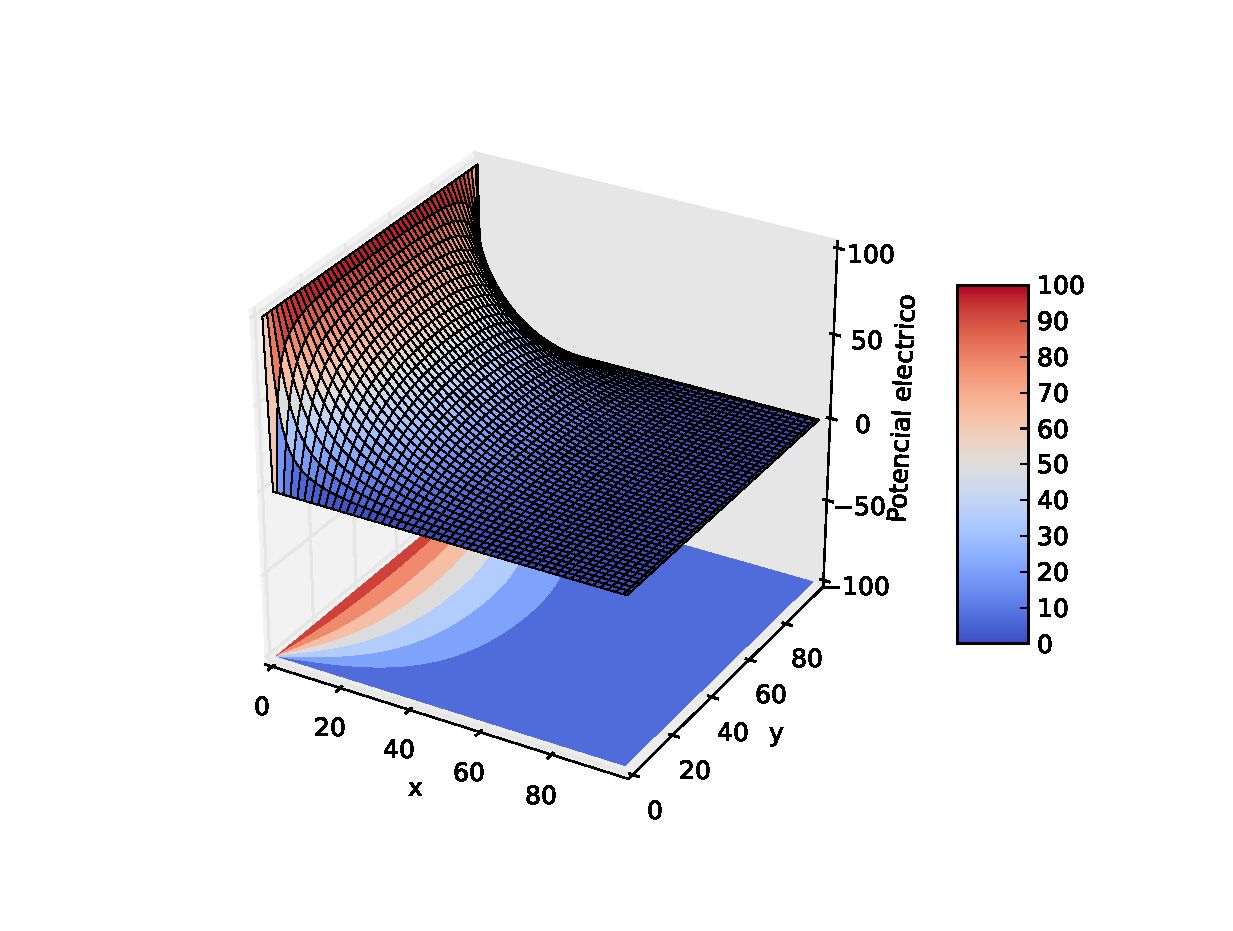
\includegraphics[scale=0.45]{Potencial01.eps} 
\end{figure}
\end{frame}
\begin{frame}
\frametitle{Primer problema para el examen}
Ahora haremos un cambio en la geometría y dificultad del problema: vamos a considerar el caso de un condensador de placas paralelas, tal como se muestra en  la siguiente figura.
\begin{center}
\begin{tikzpicture}[font=\tiny, scale=0.5]
\draw (0,0) rectangle (5,5);
\draw [line width=3pt] (1,1) -- (4,1);
\draw [line width=3pt] (1,3) -- (4,3);
\draw (5.5,2.5) node {L};
\draw (2.5,-0.5) node {L};
\draw (1,2.7) node {$100$ V};
\draw (1,1.5) node {$-100$ V};
\draw [<->](1,3.5) -- node [midway, above] {w} (4,3.5);
\draw [<->](4.2,1.1) -- node [midway, right] {d} (4.2,2.9);
\draw (0.3,0) -- (0.3,-0.3);
\draw (0,-0.3) -- (0.6,-0.3);
\draw (0.1,-0.4) -- (0.5,-0.4);
\draw (0.2,-0.5) -- (0.4,-0.5);
\end{tikzpicture}
\end{center}
\end{frame}
\begin{frame}
Tienes que resolver la ecuación para calcular el potencial en cada punto, toma en cuenta lo siguiente:
\begin{enumerate}
\item Usa un cuadro de $100 \times 100$ para tener una mejor visualización.
\item Las líneas con potencial constante, tienen una longitud $w$, tal que $w<L$  (es decir, no van de un extremo al otro)
\item Hay una separación $d$ que es constante entre las dos líneas de equipotencial.
\item Una vez con la solución de la EDP, grafica tus resultados.
\end{enumerate}
\end{frame}
\begin{frame}[fragile]
\frametitle{Solución al problema de las placas}
\begin{figure}
	\centering
	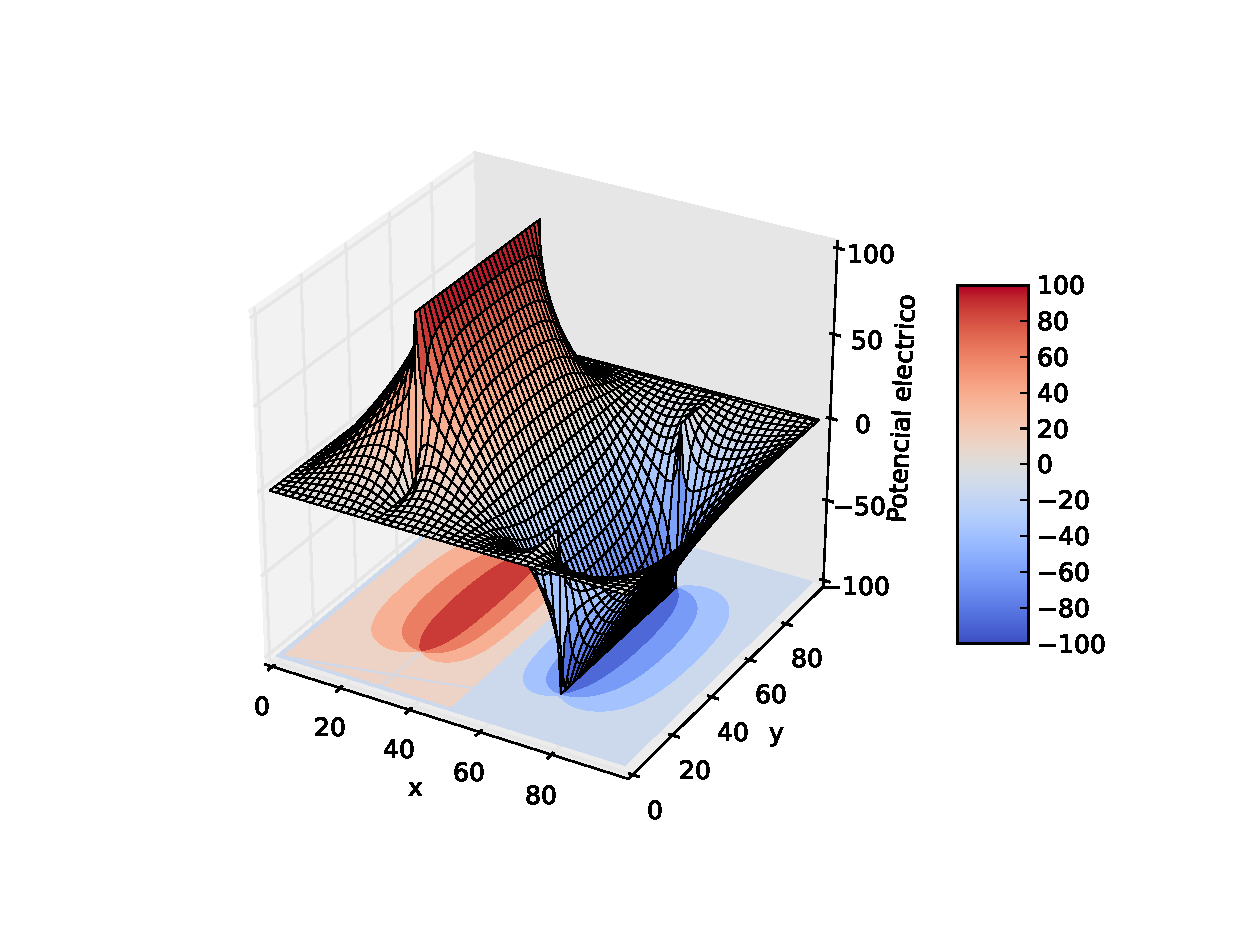
\includegraphics[scale=0.45]{Potencial02.eps} 
\end{figure}
\end{frame}
\begin{frame}
\frametitle{Segundo problema para la tarea-examen}
Resuelve la ecuación de Laplace con el siguiente arreglo donde la placa cuadrada conductora se encuentra a $1$ volt(geométricamente se localiza en el centro de la placa exterior, por lo que deberás de determinar su tamaño) mientras que la placa cuadrada exterior, se encuentra a $0$ volts.
\begin{center}
\begin{tikzpicture}
	\draw [dashed](0,0) -- (6,0);
	\draw [dashed](3,-3) -- (3,3);
	\draw [draw=black, fill=black!25](2.5,-0.5) rectangle (3.5,0.5);
	\draw (3.7,0.7) node  {$1 V$};
	\draw (0.5,-2.5) rectangle (5.5,2.5);
	\draw (5.7,2.7) node  {$0 V$};
\end{tikzpicture}
\end{center}
\end{frame}
\begin{frame}[fragile]
\begin{center}
\begin{tikzpicture}
	\draw [dashed](0,0) -- (6,0);
	\draw [dashed](3,-3) -- (3,3);
	\draw [draw=black, fill=black!25](2.5,-0.5) rectangle (3.5,0.5);
	\draw (3.7,0.7) node  {$1 V$};
	\draw (0.5,-2.5) rectangle (5.5,2.5);
	\draw (5.7,2.7) node  {$0 V$};
\end{tikzpicture}
\end{center}
Plantea dentro de tu algoritmo la solución, posteriormente presenta una gráfica e interpreta tus resultados.
\end{frame}
\begin{frame}
\frametitle{Tercer problema para la tarea-examen}
Desarrolla un esquema numérico para resolver la ecuación de Poisson
\[ \nabla^{2} \phi (r,\theta) = - \rho (r, \theta) / \epsilon_{0} \]
en coordenadas polares. Considera que la geometría en la frontera es un anillo circular con potenciales dados, para el radio interno es $\phi(a,\theta)$, y para el radio externo $\phi(b,\theta)$. Prueba tu solución asignando valores de potencial al problema.
\end{frame}
\begin{frame}
\frametitle{Tips}
La ecuación de Poisson en coordenadas polares resulta ser:
\[ \nabla^{2} \phi (r,\theta) = \dfrac{1}{r} \dfrac{\partial}{\partial r} \left( r \dfrac{\partial V}{\partial r} \right) + \dfrac{1}{r^{2}} \dfrac{\partial^{2} V}{\partial \theta^{2}} = - \dfrac{\rho(r,\theta)}{\epsilon_{0}} \]
donde $0 \leq r \leq R $ y $0 \leq \theta \leq 2 \pi$
\end{frame}
\begin{frame}[fragile]
\frametitle{Tips adicionales}
Para crear una malla en coordenadas polares, nos podemos apoyar de la siguiente manera (\emph{nota: } no es la única manera, por lo que no se confíen en que debe de ser así, les da elementos para que puedan modificar y/o ajustar esta propuesta para las necesidades del problema.
\end{frame}
\begin{frame}[fragile]
\frametitle{Primera parte}
\begin{lstlisting}
from numpy import *
import matplotlib.pylab as pp

r_a = 0.50
r_b = 1
circulos = 6  
lineas  = 20
origen = (0, 0)

for r in linspace(r_a, r_b, circulos):
    pp.gca().add_patch(pp.Circle(origen, radius=r, fill=False, color='black'))

r_ab = array([r_a, r_b])
\end{lstlisting}
\end{frame}
\begin{frame}[fragile]
\frametitle{Segunda parte}
\begin{lstlisting}
for theta in linspace(0, 2 * pi, lineas):
    pp.plot(cos(theta) * r_ab, sin(theta) * r_ab, color='red')

pp.axis('scaled')
pp.title('Creando una malla en coordenadas polares')
pp.show()
\end{lstlisting}
\end{frame}
\begin{frame}[fragile]
\frametitle{Gráfica de la malla en coordenadas polares}
\begin{figure}
\centering
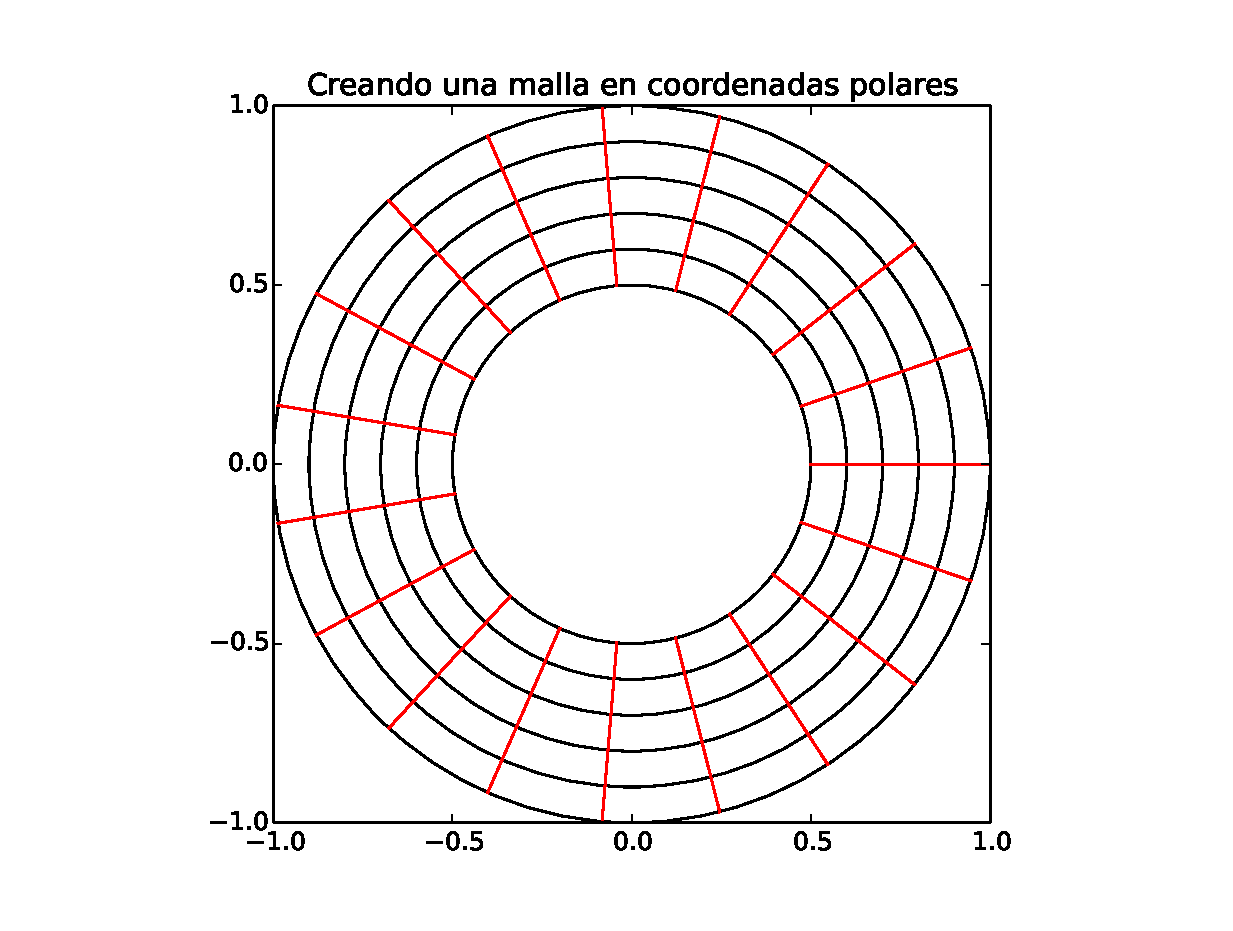
\includegraphics[scale=0.5]{Malla_Circular01.eps} 
\end{figure}
\end{frame}
\begin{frame}
Usando la malla:
\begin{eqnarray*}
r_{i} &=& i \Delta R \\
\theta &=& j \Delta \theta
\end{eqnarray*}
Se aproxima la ecuación por
\[ \begin{split}
\dfrac{1}{r_{i}} \left( r_{i+\frac{1}{2}} \dfrac{V_{i+1,j} - V_{ij}}{\Delta r} - r_{j+\frac{1}{2}} \dfrac{V_{ij}-V_{i-1,j}}{\Delta r} \right) \dfrac{1}{\Delta r} + \\
+ \dfrac{1}{r^{2}} \dfrac{V_{i,j+1}-2V_{ij}+V_{i,j-1}}{\Delta \theta^{2}} = - \dfrac{\rho(r,\theta)}{\epsilon_{0}}
\end{split} \]
\end{frame}
\begin{frame}
donde $V_{ij}$ y $r_{ij}$ son funciones
\[ (r_{i}, \theta_{j}) = (i \Delta r, j \Delta \theta) \]
Las funciones son periódicas de $j$ en la malla, con período $j=\dfrac{2 \pi}{\Delta \theta}$  y $V_{ij}$ es independiente de $j$.
\end{frame}
\end{document}
